\chapter{Implementacja modelu programowego}

W celu przetestowania wybranych algorytmów zdecydowano się wykorzystać tzw. model programowy tworzonej aplikacji. 
Do zaimplementowania prototypu wybrano komputer z~procesorem Intel Core i7 6700HQ. 
Posłużono się językiem programowania Matlab.

Z racji tego, że algorytmy miały zostać zaimplementowane z~myślą o~późniejszych przeniesieniu ich na część reprogramowalną platformy Zynq SoC.
Na jeden takt zegara otrzymuje się jeden piksel (co wynika ze sposobu obsługi sygnału wideo).
Z każdym kolejnym taktem otrzymuje się kolejne piksele. W~celu przeprowadzenie operacji kontekstowych należy korzystając z~linii opóźniających zrobić tak, aby w~danym takcie zegara mieć dostęp do wszystkich pikseli tworzących kontekst. Takie podejście powoduje, że niektóre algorytmy nie są możliwe do zaimplementowania. Należy zrezygnować ze wszystkich algorytmów, w których każdy kolejny krok algorytmu jest zależny od danych wejściowych, np. segmentacja przez rozrost. 
Z myślą o oszczędzaniu zasobów, w działaniach dzielenia starano się sprowadzać mianownik do potęgi liczby 2.
Taką operację można wtedy wykonać przy wykorzystaniu dużo mniejszej ilości zasobów układu FPGA.  

Aplikacja ma na celu detekcję punktów reprezentujących prawą i lewą linie drogową. 

\section{Binaryzacja}
W celu otrzymania obrazu binarnego z~obrazu w~formacie RGB zdecydowano się wykorzystać binaryzację stałym progiem \cite{1}. 
Obraz wejściowy najpierw konwertowany jest w~obraz w~skali szarości. Otrzymano wykorzystując składową L z formatu HSL. Wzór na przekształcenie składowych RGB w składową L \eqref{eq:hsl}. 

\begin{equation}
{\displaystyle {\begin{aligned}\,C_{max}\,=\,max(R,\,G,\,B)\\[10pt]\,C_{min}\,=\,min(R,\,G,\,B)\\[10pt]\,L\,=(C_{max}\,+\,C_{min})\,/\,2\end{aligned}}}\\[10pt]
\label{eq:hsl}
\end{equation}

Po otrzymaniu obrazu w skali szarości jest on poddawany binaryzacji progiem o wartości 192, jest to około 3/4 maksymalnej wartości jaką może posiadać piksel.
Podany prób sprawdzał się wystarczająco w celu oddzielenia pasów od jezdni. 
Rysunek \ref{fig:im_color} przedstawia obraz wejściowy w kolorze. Rysunek \ref{fig:im_grey} obraz w~skali szarości. Rysunek \ref{fig:in_ROI} prezentuje obszar wyjściowy, po procesie binaryzacji podanym progiem.

\begin{figure}[h]
	\centering
	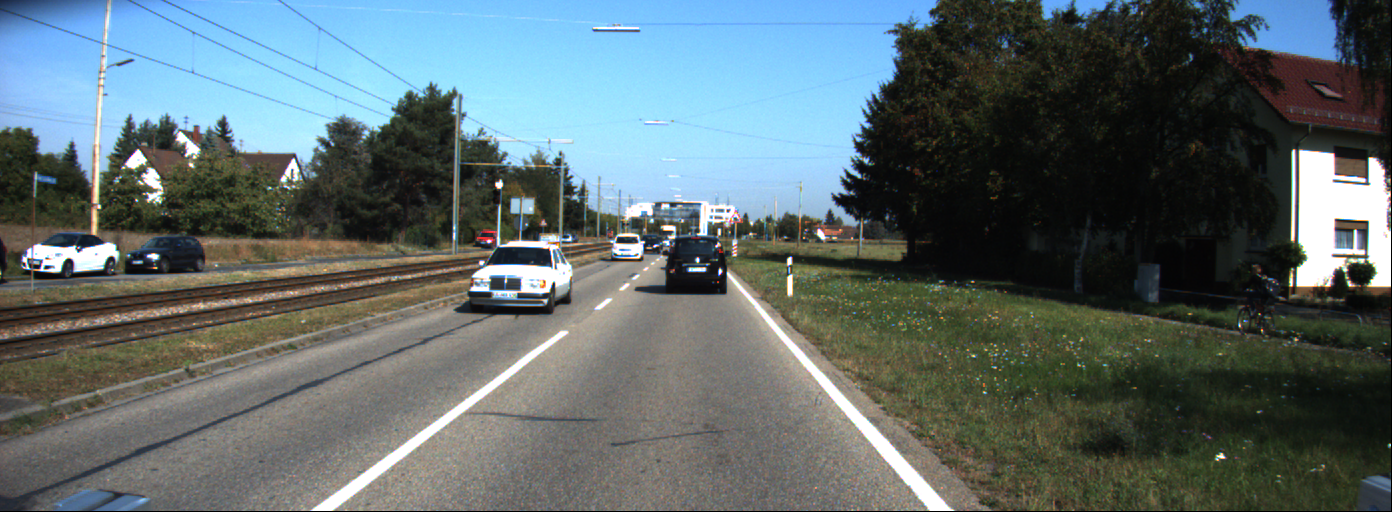
\includegraphics[scale=0.3]{obraz_color.png}
	\caption{Obraz wejściowy przed przekształceniami}
	\label{fig:im_color}
\end{figure}
\begin{figure}[h]
	\centering
	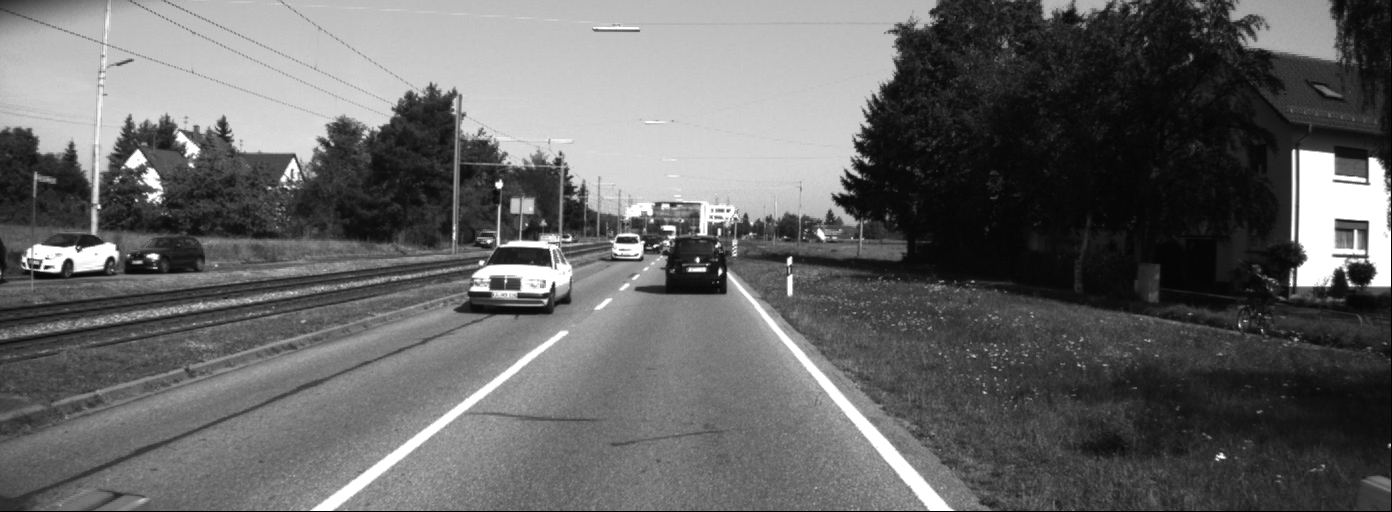
\includegraphics[scale=0.3]{obraz_grey.png}
	\caption{Obraz w skali szarości}
	\label{fig:im_grey}
\end{figure}
\begin{figure}[h]
	\centering
	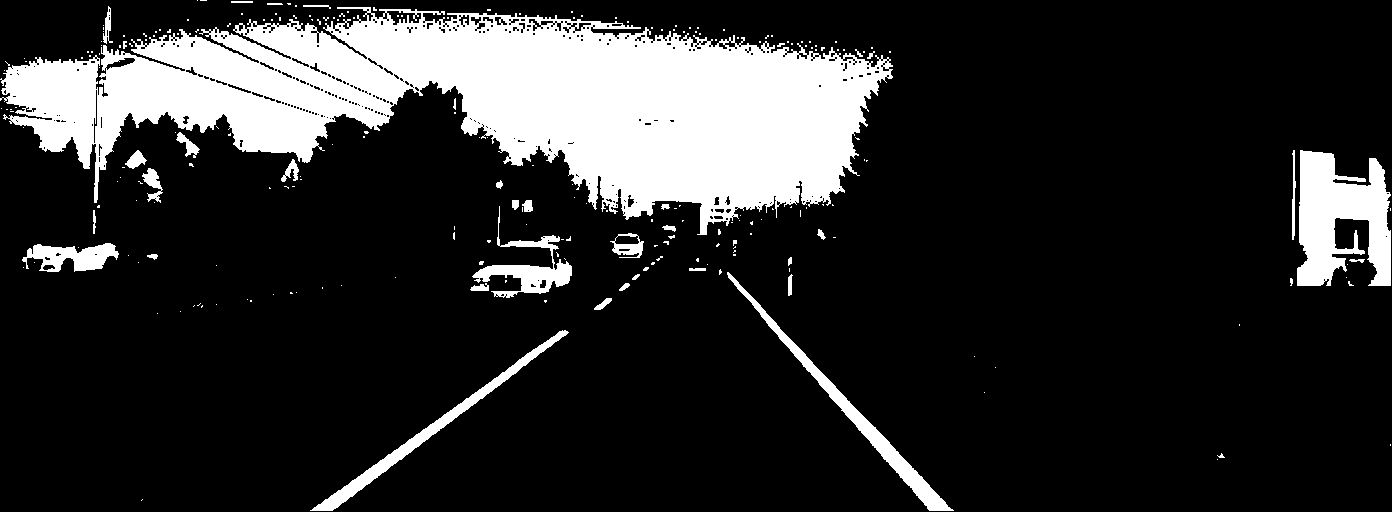
\includegraphics[scale=0.3]{obraz_binarny.png}
	\caption{Obraz binarny przed wyznaczeniem ROI w modelu programowym}
	\label{fig:in_ROI}
\end{figure}
\section{ROI}
Celem wyznaczenia ROI jest pozbycie się części danych obrazu, które mogą utrudniać dalszą detekcję pasów ruchu drogowego.
Obszar zainteresowanie został wyznaczony statycznie przy pomocy dobranych ograniczeń.
Aby piksel nie został odfiltrowany, czyli jego wartość ustawiona na 0, jego współrzędne muszą spełniać warunki opisane wzorami \eqref{eq:ROI1}. Przy czym $x$ oznacza numer kolumny, w~której znajduje się piksel, a~$y$ numer wiersza. $Width$ oznacza szerokość obrazu, a $High$ wysokość obrazka.
Ograniczenia zostały dobrane w taki sposób, aby odfiltrować jak najwięcej tła obrazu i pozostawić praktycznie tylko obiekt pierwszoplanowy, którym jest jezdnia.
Ze względu na znane standardy szerokości pasów ruchu drogowego, zdecydowano się statycznie dobierać ograniczenia.

\begin{equation}
{\displaystyle {\begin{aligned}\,x\,-\,3/8 \,Width\,<\,y\\[10pt]\,-x\,+\,5/8 \,Width\,<\,y\\[10pt]\,y\,>\,1/2 \,High\end{aligned}}}\\[10pt]
\label{eq:ROI1}
\end{equation}


Algorytm wyznaczania ROI należy przeprowadzić po wcześniejszym zbinaryzowaniu obrazu. 
Przy poprawnej binaryzacji linie drogowe zostają zaliczane jako obiekt pierwszoplanowy (białe piksele).
Za to jezdnia jest zaliczana jako obiekt drugoplanowy (czarne piksele).
Przeprowadzenie kolejno metody wyznaczania ROI powoduje usunięcie obszaru znajdującego się poza pasem ruchu.
Rysunek \ref{fig:in_ROI} przedstawia obraz wejściowy, zbinaryzowane zdjęcie drogi. Rysunek \ref{fig:out_ROI} obraz wyjściowy, obraz po wyznaczeniu ROI.
Rysunek \ref{fig:out_ROI_mask} prezentuje obszar (czarny), który zostaje usunięty z~obrazu w wyniku wyznaczania ROI.


\begin{figure}[h]
	\centering
	
\includegraphics[scale=0.3]{obraz_roi.png}
	\caption{Obraz wyjściowy wyznaczania ROI w modelu programowym}
	\label{fig:out_ROI}
\end{figure}
\begin{figure}[h]
	\centering
	
\includegraphics[scale=0.3]{roi.png}
	\caption{Obraz przedstawiający, która cześć obrazu nie została usunięta (białe piksele) podczas wyznaczania ROI. }
	\label{fig:out_ROI_mask}
\end{figure}


\section{LMPS}
LMPS (ang. \textit{Lane Marker Pattern Search} -- wyszukiwanie wzorców pasów ruchu) zaimplementowano tak, aby obiekty nienależące do zbioru linii drogowych zostały odfiltrowane. 
Takimi elementami są między innymi pasy przejścia dla pieszych oraz przedmioty znajdujące się na ulicy. 
Przed użyciem filtru LMPS, na obrazku przeprowadzamy operację zamknięcia w celu uniknięcia błędnego nie rozpoznania pasów wyniku ich zużycia bądź zabrudzenia. Pozbywamy się czarnych pikseli z wnętrza obiektów.
Na~rysunkach \ref{fig:out_ROI} i~\ref{fig:img_1_lmps} został przedstawiony efekt odfiltrowania pasów. 
Na obrazie wynikowym znajdują białe piksele odnoszą się do wykrytych linii drogowych. 
Algorytm działa na zasadzie sprawdzania grubości w~poziomie białych części obrazu wejściowego. 
Przyjęto, że linie drogowe mają konkretną grubość oraz wzięto pod uwagę wpływ perspektywy na zniekształcenie obiektów. 
Dzięki temu progi określające szerokość linii drogowej przedstawionej na obrazie zmieniają się liniowo w~zależności od obecnego indeksu wiersza piksela.

\begin{figure}[h]
	\centering
	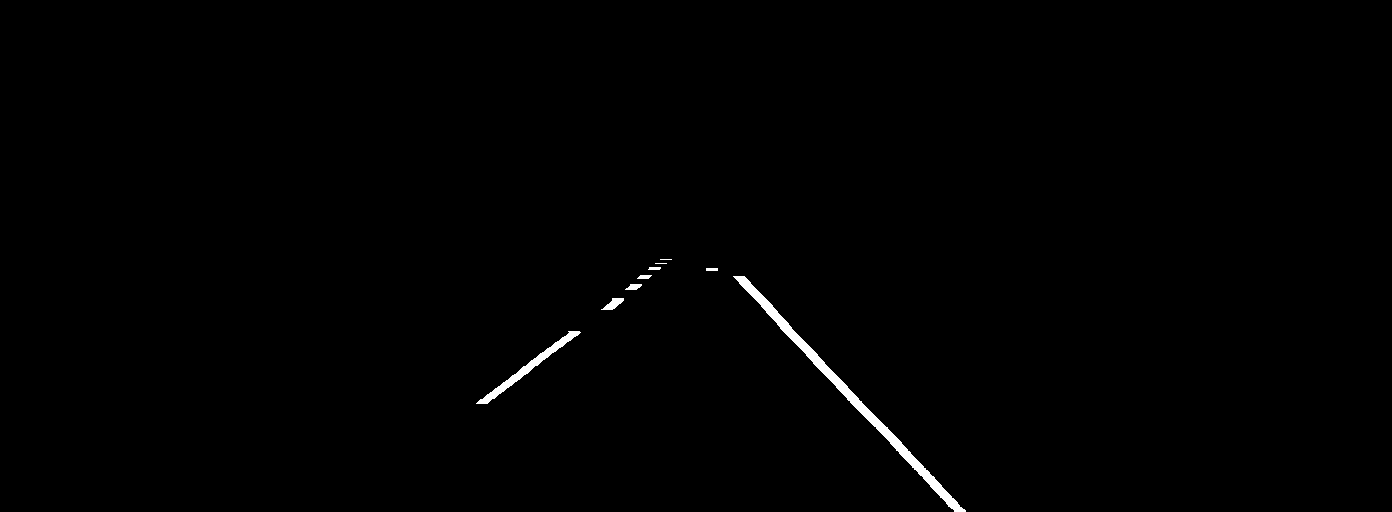
\includegraphics[scale=0.3]{obraz_lmps.png}
	\caption{Obraz \ref{fig:in_ROI} przetworzony przez filtr LMPS}
	\label{fig:img_1_lmps}
\end{figure}


\section{Podział obrazu i wyznaczenie wykrytych linii}

Kolejnym etapem detekcji pasa ruchu 
Obraz został podzielony na osiem części. Podział przedstawiony jest na grafice \ref{fig:ograniczenia}.
W~każdym z~obszarów został wyznaczony środek ciężkości obliczony przy pomocą wzorów \eqref{eq:sc_11} - \eqref{eq:sc_15}. Bazują one na momentach geometrycznych figur. Z czego figura jest rozumiana jako zbiór pikseli o takiej sam wartości.
Uzyskane punkty stanowią podstawę do wyznaczenia krzywych reprezentujących wykryte linie drogowe. Punkty wykryte w obszarach z prawej strony zostały wykorzystane do reprezentacji prawej linii drogowej. Analogicznie postąpiono z punktami wykrytymi po lewej stronie obrazka, które wykorzystamy do otrzymania krzywej reprezentującą lewą linię drogową/

\begin{figure}
	\centering
	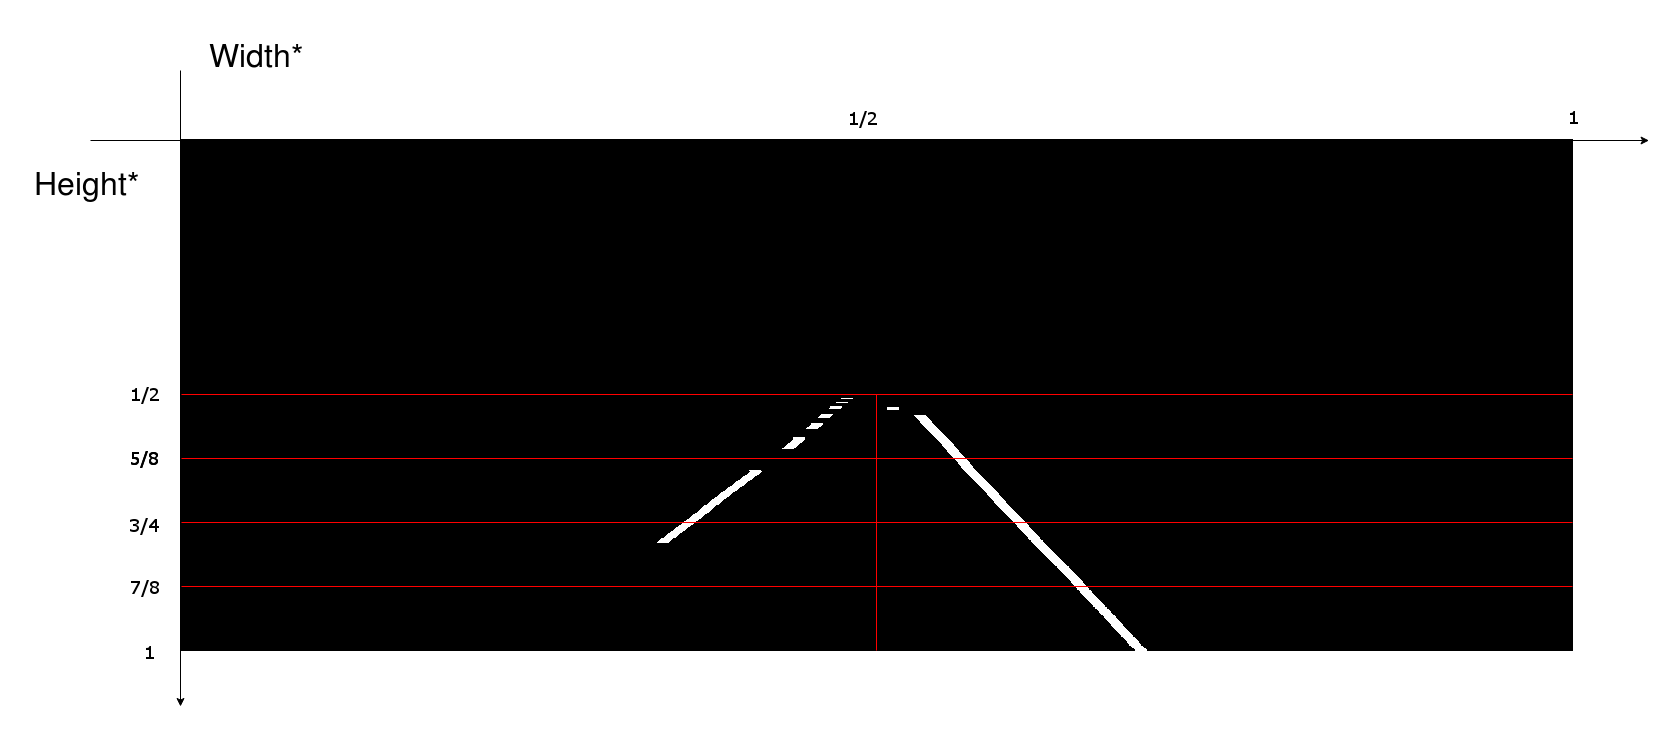
\includegraphics[scale=0.3]{ograniczenia.png}
	\caption{Zdjęcie przedstawiające wydzielone obszary, w których szukane są środki ciężkości.} 
	\label{fig:ograniczenia}
\end{figure}

\noindent Gdzie $Width$ -- szerokość obrazu w pikselach, $Height$ -- Wysokość obrazu


\begin{equation}
m_{00}={\sum _{i=0}^{N-1}}{\sum _{j=0}^{M-1}x_{ij}}\\[10pt]
\label{eq:sc_11}
\end{equation}
\begin{equation}
m_{10}={\sum _{i=0}^{N-1}}{\sum _{j=0}^{M-1}i \cdot x_{ij}}\\[10pt]
\label{eq:sc_12}
\end{equation}
\begin{equation}
m_{01}={\sum _{i=0}^{N-1}}{\sum _{j=0}^{M-1}j \cdot x_{ij}}\\[10pt]
\label{eq:sc_13}
\end{equation}
\begin{equation}
x_{sc}={\frac {m_{10}}{m_{00}}}\\[10pt]
\label{eq:sc_14}
\end{equation}
\begin{equation}
y_{sc}={\frac {m_{01}}{m_{00}}}\\[10pt]
\label{eq:sc_15}
\end{equation}

\noindent Gdzie: $m_{00}, m_{10}, m_{01}$ -- zmienne pomocnicze, $i$ -- indeks wiersza piksela, $j$ -- indeks kolumny obecnego piksela, $i$ -- indeks kolumny piksela, $x_{ij}$ -- piksel o współrzędnych $i$, $j$, $N$ -- szerokość obrazu, $M$ -- wysokość obrazu, $x_{sc}$ -- współrzędna wierszowa punktu reprezentującego środek ciężkości, $y_{sc}$ - współrzędna kolumnowa punktu reprezentującego środek ciężkości.

\begin{figure}[h]
	\centering
	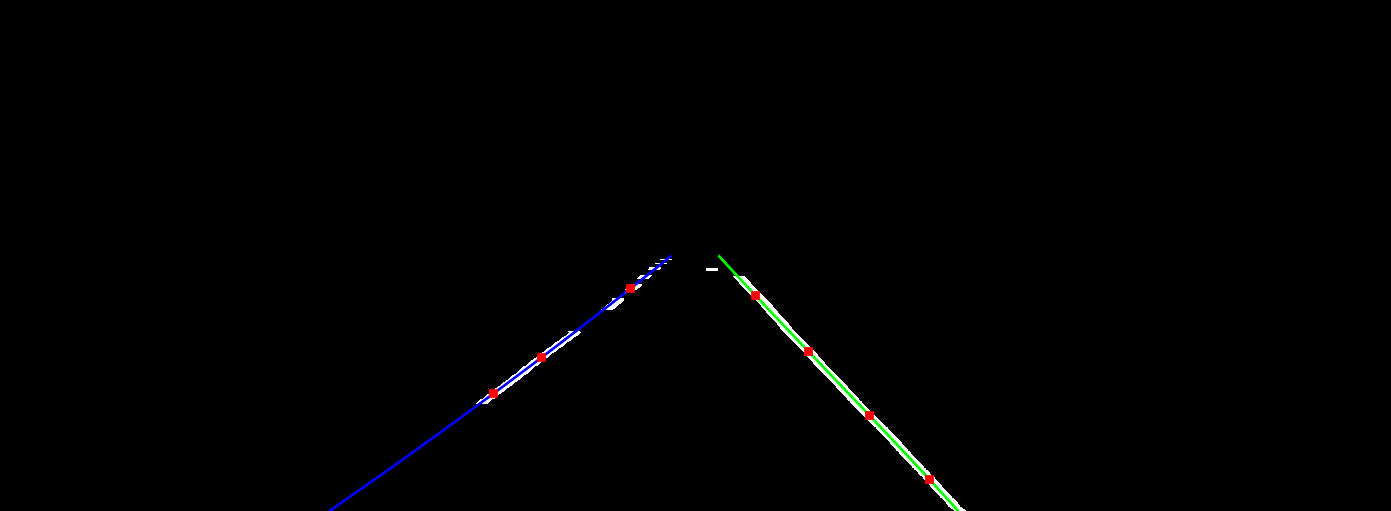
\includegraphics[scale=0.3]{krzywe.png}
	\caption{Obraz przedstawiający wyznaczone środki ciężkości, reprezentowane są przez czerwone punkty. Oraz łączące je proste}
	\label{fig:mass_centers1}
\end{figure}

Na rysunku \ref{fig:mass_centers1} przedstawiono punkty oznaczające wyznaczone środki ciężkości, oraz łączącą ją krzywą.
Znalezione czerwone punkty leżą na liniach otrzymanych z filtru LMPS. 
Dopasowane krzywe pokrywają się z~liniami. 